\documentclass[a4paper,12pt]{report}
\usepackage[left=2cm,right=2cm,top=2cm,bottom=2cm]{geometry}
\usepackage[utf8]{inputenc}
\usepackage{graphicx}
\usepackage{eso-pic}
\usepackage{transparent}
\usepackage{xcolor}
\usepackage{floatrow}
\usepackage{tabularx}
\usepackage{listings}
\usepackage{xcolor}
\usepackage{caption}

\newcommand{\LogoPath}{RUET_logo.png}

\definecolor{odp-background}{RGB}{40, 44, 52}
\definecolor{odp-text}{RGB}{171, 178, 191}
\definecolor{odp-keyword}{RGB}{249, 38, 114}
\definecolor{odp-comment}{RGB}{98, 114, 164}
\definecolor{odp-string}{RGB}{152, 195, 121}
\definecolor{odp-number}{RGB}{174, 129, 255}
\definecolor{odp-function}{RGB}{189, 147, 249}

\lstdefinestyle{cppstyle}{
    language=C++,
    basicstyle=\color{odp-text}\ttfamily\small,
    keywordstyle=\color{odp-keyword},
    commentstyle=\color{odp-comment},
    stringstyle=\color{odp-string},
    numbers=left,
    numberstyle=\tiny\color{odp-number},
    stepnumber=1,
    numbersep=5pt,
    backgroundcolor=\color{gray!5},
    frame=single,
    rulecolor=\color{odp-text},
    breaklines=true,
    breakatwhitespace=true,
    tabsize=4,
    moredelim=[s][\color{odp-header}]{\#include\ <}{>}, % Header files included in #include <>
    otherkeywords={!,!=,~,$,*,\&,\%,:,\#, ifndef, define, endif, include},
    emph={!,!=,~,$,*,\&,\%,:,\#},
    emphstyle=\color{odp-function}
}

\begin{document}
\begin{titlepage}
    \begin{center}

        \AddToShipoutPicture*{\put(0.125\paperwidth,0.125\paperheight){
                \transparent{0.1}
                \includegraphics*[width=0.75\paperwidth,height=0.75\paperheight,keepaspectratio]{RUET_logo.png}%
            }
        }
        \textbf{\textcolor{yellow}{\rmfamily Haven's Light is Our Guide}}

        \begin{figure}[h]
            \transparent{0.8}
            \centering
            \includegraphics[width=0.3\textwidth]{\LogoPath}
        \end{figure}

        \vspace*{0in}
        \Large
        \textbf{\mbox{Rajshahi University of Engineering \& Technology}}
        \large
        \textbf{\mbox{\textcolor{blue}{Department of Computer Science \& Engineering}}}

        \vfill
        \Huge
        \textbf{\mbox{Lab Report}}
        \vfill

        \begin{table}[h]
            \centering
            \begin{tabularx}{0.7\paperwidth}{|c|X|}
                \hline
                \textbf{Course Code:}     & CSE 2204                                                                                 \\
                \hline
                \textbf{Course Title:}    & Numerical Methods Sessional                                                              \\
                \hline
                \textbf{Experiment No:}   & 03                                                                                       \\
                \hline
                \textbf{Experiment Name:} & Exploring Functional Values through Newton's Forward and Backward Interpolation Formula. \\
                \hline
            \end{tabularx}
        \end{table}

        \vspace{0.5in}
        \textbf{Date:} \\
        \today

        \vfill

        \begin{table}[h]
            \centering
            \begin{tabularx}{0.7\paperwidth}{|X|X|}
                \hline
                Submitted By:               & Submitted To:                                    \\
                \hline
                Name: Md. Abdullah Al Mamun & Shyla Afroge                                     \\
                \hline
                Section: A                  & Assistant Professor                              \\
                \hline
                Roll No: 2003028            & Computer Science \& Engineering                  \\
                \hline
                Year: 2nd Year Odd Semester & Rajshahi University of Engineering \& Technology \\
                \hline
            \end{tabularx}
        \end{table}
    \end{center}
\end{titlepage}

\section*{Experiment No: 03}
\section*{Experiment Name: \small Exploring Functional Values through Newton's Forward and Backward Interpolation Formula.}
\section*{Theory:}

\subsection*{Newton's Forward Interpolation Formula:}
\qquad Given a set of data points $(x_0, y_0), (x_1, y_1), \ldots, (x_n, y_n)$ with a common difference $h = x_1 - x_0$, Newton's Forward Interpolation Formula estimates $y$ at a point $x$ within the range $(x_0, x_n)$ as follows: \[ y = y_0 + t \Delta y_0 + \frac{t(t-1)}{2!} \Delta^2 y_0 + \ldots + \frac{t(t-1)\ldots(t-n+1)}{n!} \Delta^n y_0 \] where $t = \frac{x - x_0}{h}$ and $\Delta y_i = y_{i+1} - y_i$ are the finite differences.

\subsection*{Algorithm:}
\begin{enumerate}
    \item \textbf{Calculate Finite Differences:}
          \begin{itemize}
              \item Calculate first-order differences: $\Delta y_i = y_{i+1} - y_i$ for $i = 0, 1, \ldots, n-1$.
              \item Calculate second-order differences: $\Delta^2 y_i = \Delta y_{i+1} - \Delta y_i$ for $i = 0, 1, \ldots, n-2$.
              \item Continue this process up to the $n$-th order differences.
          \end{itemize}
    \item \textbf{Calculate Coefficients:}
          \begin{itemize}
              \item Initialize coefficients $a_0 = y_0$.
              \item For $k = 1, 2, \ldots, n$, calculate $a_k = \frac{\Delta^k y_0}{k!}$.
          \end{itemize}
    \item \textbf{Interpolation Formula:}
          \begin{itemize}
              \item The interpolated value at a point $x$ is given by the formula:
                    \[ P(x) = a_0 + a_1 t + a_2 t(t-1) + \ldots + a_n t(t-1)\ldots(t-n+1) \]
                    where $t = \frac{x - x_0}{h}$.
          \end{itemize}
\end{enumerate}

\subsection*{Newton's Backward Interpolation Formula:}
\qquad When the data points are given in equally spaced intervals but in reverse order, Newton's Backward Interpolation Formula estimates $y$ at a point $x$ within the range $(x_0, x_n)$ as follows: \[ y = y_n + t \Delta y_n + \frac{t(t+1)}{2!} \Delta^2 y_n + \ldots + \frac{t(t+1)\ldots(t+n-1)}{n!} \Delta^n y_n \] where $t = \frac{x - x_n}{h}$ and $\Delta y_i = y_i - y_{i-1}$. These interpolation formulas are valuable tools when evenly spaced data points are available, and the choice between forward and backward interpolation depends on the arrangement of the given data points.

\subsection*{Algorithm:}
\begin{enumerate}
    \item \textbf{Calculate Finite Differences:}
          \begin{itemize}
              \item Calculate first-order differences: $\Delta y_i = y_i - y_{i-1}$ for $i = 1, 2, \ldots, n$.
              \item Calculate second-order differences: $\Delta^2 y_i = \Delta y_i - \Delta y_{i-1}$ for $i = 2, 3, \ldots, n$.
              \item Continue this process up to the $n$-th order differences.
          \end{itemize}
    \item \textbf{Calculate Coefficients:}
          \begin{itemize}
              \item Initialize coefficients $a_n = y_n$.
              \item For $k = 1, 2, \ldots, n$, calculate $a_{n-k} = \frac{\Delta^k y_n}{k!}$.
          \end{itemize}
    \item \textbf{Interpolation Formula:}
          \begin{itemize}
              \item The interpolated value at a point $x$ is given by the formula:
                    \[ P(x) = a_n + a_{n-1} t + a_{n-2} t(t+1) + \ldots + a_0 t(t+1)\ldots(t+n-1) \]
                    where $t = \frac{x - x_n}{h}$.
          \end{itemize}
\end{enumerate}

\section*{Program:}

\begin{lstlisting}[style=cppstyle, caption={Newton’s Forward Interpolation}, label={lst:cppcode}, basicstyle=\fontsize{10}{10}\selectfont\ttfamily]
    double NewtonForward(double x[], double y[], int n, double p)
    {
        double dely[n][n], a = x[0], h = x[1] - x[0], u, y0;
    
        for (int i = 0; i < n; i++)
            dely[i][0] = y[i];
    
        for (int i = 1; i < n; i++)
            for (int j = 0; j < n - i; j++)
                dely[j][i] = dely[j + 1][i - 1] - dely[j][i - 1];
    
        int k = 0;
        while (a - p > h)
        {
            a = x[k];
            k++;
        }
        u = (p - a) / h;
        y0 = dely[0][0];
        double tempU = u;
    
        for (int i = 1; i < (n - k); i++)
        {
            if (i != 1)
                tempU = tempU * (u - i + 1);
    
            tempU = tempU / (double)i;
            y0 += tempU * dely[k][i];
        }
        return y0;
    }
\end{lstlisting}

\begin{lstlisting}[style=cppstyle, caption={Newton’s Backward Interpolation}, label={lst:cppcode}, basicstyle=\fontsize{10}{10}\selectfont\ttfamily]
    double NewtonBackward(double x[], double y[], int n, double p)
    {
        double dely[n][n], a = x[n - 1], h = x[1] - x[0], u, y0;
    
        for (int i = 0; i < n; i++)
            dely[i][0] = y[i];
    
        for (int i = 1; i < n; i++)
            for (int j = 0; j < n - i; j++)
                dely[j][i] = dely[j + 1][i - 1] - dely[j][i - 1];
    
        int k = 0;
        while (a - p > h)
        {
            a = x[k];
            k++;
        }
        u = (p - a) / h;
        y0 = dely[n - 1][0];
        double tempU = u;
    
        for (int i = 1; i < (n - k); i++)
        {
            if (i != 1)
                tempU = tempU * (u + i - 1);
    
            tempU = tempU / (double)i;
            y0 += tempU * dely[n - k - i - 1][i];
        }
        return y0;
    }
\end{lstlisting}

\begin{lstlisting}[style=cppstyle, caption={Main Program}, label={lst:cppcode}, basicstyle=\fontsize{10}{10}\selectfont\ttfamily]
    #include <iostream>
    using namespace std;
    
    void takeInput(double *x, double *y, int &n, double &x0)
    {
        cout << "Enter the number of data points: ";
        cin >> n;
        cout << "Enter the values of x: ";
        for (int i = 0; i < n; i++)
            cin >> x[i];
    
        cout << "Enter the values of y: ";
        for (int i = 0; i < n; i++)
            cin >> y[i];
        cout << endl;
    
        cout << "Enter the value of x for which y is to be found: ";
        cin >> x0;
    }
    
    int main()
    {
        int input = 0;
        while (input != 3)
        {
            // take all the inputs
            int n = 0;
            double x[10000], y[10000], x0;
    
            // take the choice
            cout << "1. Newton Forward" << endl;
            cout << "2. Newton Backward" << endl;
            cout << "3. Exit" << endl
                 << endl;
            cout << "Note: All the data must be equally spaced" << endl;
            cout << "Enter your choice: ";
            cin >> input;
            cout << endl;
    
            switch (input)
            {
            case 1:
            {
                takeInput(x, y, n, x0);
                double y0 = NewtonForward(x, y, n, x0);
                cout << "The value of y at x = " << x0 << " is " << y0 << endl
                     << endl
                     << endl;
                break;
            }
            case 2:
            {
                takeInput(x, y, n, x0);
                double y0 = NewtonBackward(x, y, n, x0);
                cout << "The value of y at x = " << x0 << " is " << y0 << endl
                     << endl
                     << endl;
                break;
            }
            case 3:
            {
                return 0;
            }
            default:
            {
                cout << "Invalid choice" << endl;
                break;
            }
                cout << endl
                     << endl;
            }
        }
    }
\end{lstlisting}

\section*{Result:}
\qquad Newton's Forward and Backward Interpolation Formulas are methods for estimating values between known data points through polynomial interpolation. Forward Interpolation assumes equally spaced data from left to right, using forward finite differences. Backward Interpolation is for right-to-left data with backward finite differences. Both involve systematic finite difference and coefficient calculations, providing efficient interpolation. The choice depends on data arrangement, with forward for left-to-right and backward for right-to-left data. Despite directional distinctions, both share the same principles and are valuable for accurately estimating values within a given data range.

\begin{figure}[H]
    \centering
    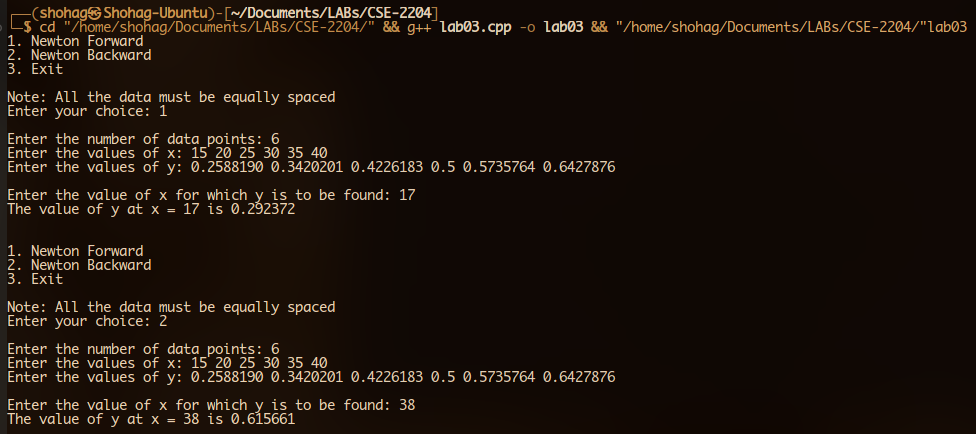
\includegraphics[width=0.87\textwidth]{result.png}
    \caption{Output of the Program}
    \label{fig:result}
\end{figure}

\end{document}